% Chapter Template

\chapter{Related Literature} \label{relatedLiterature} % Main chapter title

\label{2.} % Change X to a consecutive number; for referencing this chapter elsewhere, use \ref{ChapterX}

%----------------------------------------------------------------------------------------
%	SECTION 1
%----------------------------------------------------------------------------------------

\section{Anomaly or Outlier?} \label{anomalies}

Generally, there is no agreement on how to distinguish between anomalies and outliers. The following often used citation claims equality of the term outliers and anomalies.\\

\noindent\enquote{\itshape Outliers are also referred to as abnormalities, discordants, deviants, or anomalies in the data mining
	and statistics literature.} - Aggarwal \parencite*{Aggarwal2013}\\

By others, outliers are regarded as corruption in data, while anomalies are abnormal points with a particular pattern. 
In the context of this paper, only the term anomaly is used to refer to such irregular behaviour. It is hereby important to provide a clear definition for the concept of anomaly. This is critical since different meanings of abnormalities necessitate different detection methods. As a result, it is important to identify the key characteristics of anomalies and to use the description to highlight the boundaries. Following, two common definitions of anomalies:\\

\noindent\enquote{\itshape Anomalies are patterns in data that do not conform to a well-defined notion of normal behaviour.} - Chandola et al. \parencite*{Chandola2009}\\

Ord \parencite*{Ord1996}, defines anomalies as follows:\\

\noindent\enquote{\itshape An observation (or subset of observations) which appears to be inconsistent with the remainder of that set of data.}\\

Anomalies have two major features, according to both definitions:

\begin{itemize}
	\item The anomalies' distribution deviates significantly from the data's overall distribution.
	\item Standard data points make up the vast majority of the dataset. The anomalies make up a very small portion of the overall dataset.
\end{itemize}

The development of anomaly detection methods is dependent on these two factors. The second property prevents the employment of common classification methods that depend on balanced datasets.

\subsection{Types of Anomalies}
Anomalies come in a variety of shapes and sizes. Braei and Wagner \parencite*{Braei2020}  divide the anomalies into three categories:

\begin{enumerate}
	\item \textbf{Point Anomalies} - A point anomaly occurs when a single point deviates dramatically from the rest of the data.
	A point anomaly in a time series is, for example, a temperature peak in an otherwise, over time, steady temperature.
	\item \textbf{Collective Anomalies} - Individual points may or may not be anomalous, but a series of points may be. A time series example could look as follows: A bank customer withdraws \$500 from her account per weekday. Although withdrawing \$500 every now and then is common for the consumer, a series of withdrawals is unusual.
	\item \textbf{Contextual Anomalies} - Some points can appear natural in one context but be identified as anomalous in another: In Germany, a daily temperature of 35 degrees Celsius is considered natural in the summer, but the same temperature in the winter is considered unusual.
\end{enumerate}

Knowing ahead of time what kind of anomaly the data might contain helps the data analyst choose the best detection process. Some methods for detecting point anomalies fail to detect collective or contextual anomalies entirely \parencite{Braei2020}. 

%\subsection{Time Series Patterns}
%
%There are a few key characteristics of time-series that are briefly described here.
%
%\subsubsection{Level}
%
%The mean of the series is used to determine the time-series standard. When a time-series has a pattern, the level is also said to be changing.
%
%\subsubsection{Trend}
%
%If the mean of a time series does not remain constant over time but increases or decreases, it is said to have a trend. A pattern can be either linear or non-linear in nature. Figure 3 shows a positive trend from 2005 to 2008, and then a downward trend after that.
%
%\begin{figure}[h]
%	\centering
%	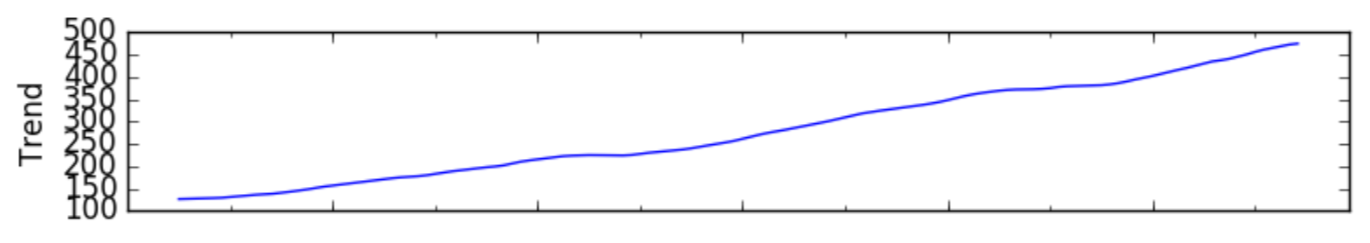
\includegraphics[scale=0.3]{Figures/Trend}
%	\decoRule
%	\caption[Trend]{Trend \parencite{}}
%	\label{fig:Trend}
%	%https://medium.com/swlh/time-series-analysis-7006ea1c3326
%\end{figure}
%
%\subsubsection{Seasonality}
%
%Seasonality refers to the occurrence of variations on a regular basis. Seasonal variables such as the time of year, day of the week, and other similarities influence the time-series, which is why it is called seasonal. As a result, it has a set period of time that is often limited to a year. A seasonal time-series is depicted in Figure 4 \parencite{Braei2020}.
%
%\begin{figure}[h]
%	\centering
%	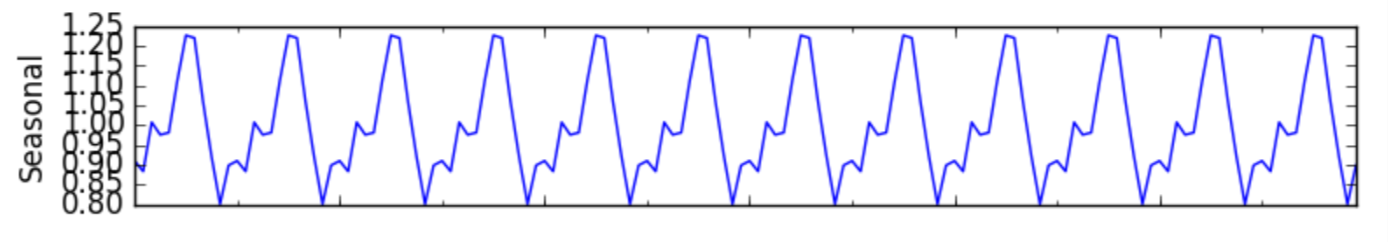
\includegraphics[scale=0.3]{Figures/Seasonal}
%	\decoRule
%	\caption[Seasonality]{Seasonality \parencite{}}
%	\label{fig:Seasonality}
%	%https://medium.com/swlh/time-series-analysis-7006ea1c3326
%\end{figure}
%
%\subsubsection{Noise}
%
%The variability in the observations that the model cannot account for.
%
%\begin{figure}[h]
%	\centering
%	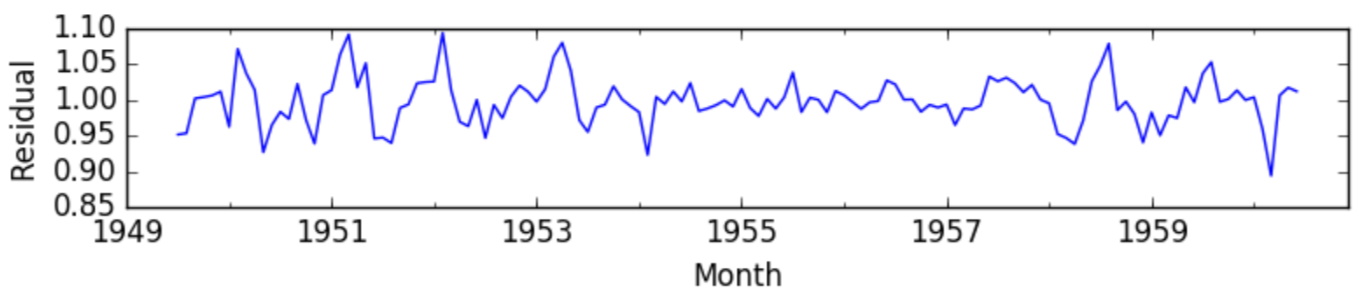
\includegraphics[scale=0.3]{Figures/Residual}
%	\decoRule
%	\caption[Noise]{Noise \parencite{}}
%	\label{fig:Noise}
%	%https://medium.com/swlh/time-series-analysis-7006ea1c3326
%\end{figure}
%
%\subsubsection{Observed}
%
%All the above componenents combined could provide the observed time series shown in Figure . The components may add up to form a model such as: 
%
%\begin{equation}
%	Y =level + trend + seasonality + noise
%\end{equation}
%
%\begin{figure}[h]
%	\centering
%	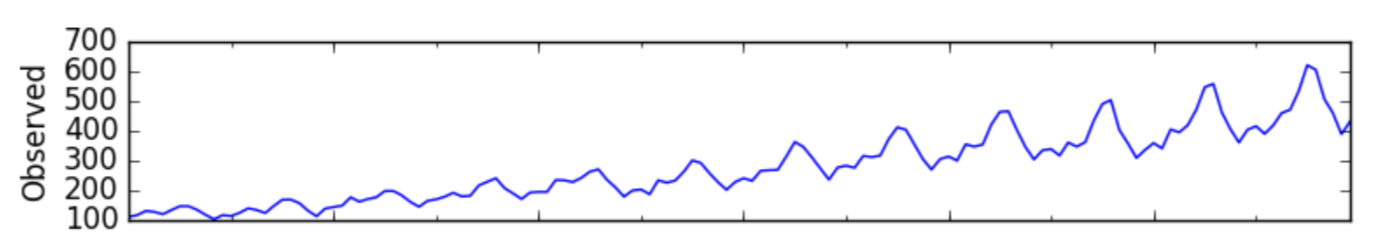
\includegraphics[scale=0.3]{Figures/Observed}
%	\decoRule
%	\caption[Observed]{Observed \parencite{}}
%	\label{fig:Observed}
%	%https://medium.com/swlh/time-series-analysis-7006ea1c3326
%\end{figure}

\section{Anomaly Detection on Univariate Time Series} \label{Anomaly Detection on Univariate Time Series}

First, anomaly detection on univariate time series using deep learning approaches is investigated to gain insight into the used architecture and the overall training and detection process. 

\subsection{Univariate Anomaly detection with LSTM}

Because of their ability to retain long term memory, Long Short Term Memory (LSTM) networks have been shown to be especially useful for learning sequences containing longer term patterns. Malhotra et al. \parencite*{Malhotra2015} model normal behaviour with a predictor and then use the prediction errors to classify abnormal behaviour. This is especially useful in real-world anomaly detection scenarios where instances of normal behaviour are plentiful, but instances of anomalous behaviour are rare. For prediction, multiple time steps into the future are forecasted to ensure that the networks capture the temporal structure of the chain. As a result, each point in the series has multiple corresponding expected values made at various points in the past, resulting in multiple error values. The likelihood of normal behaviour on the test data is calculated using the probability distribution of the errors produced when predicting on normal data. For this approach Malhotra et al. \parencite{Malhotra2015} use a deep LSTM neural networks. The proposed network architecture with two hidden layers is successfully applied on different univariate time series such Electrocardiograms (ECG), a valve time series and a power demand dataset. The proposed approach on univariate data could easily be adopted with multivariate data, where instead of a univariate in- and output, a multivariate data set is fed into the neural network to predict a multivariate output. 

Malhotra et. al \parencite*{Malhotra2015} use an interesting split of the dataset to train the neural networks. The data was divided into four sets. a non-anomalous training set, a non-anomalous validation set, a mixture of anomalous and non-anomalous validation set and test set, also consisting of an anomalous and non-anomalous sequences. This approach was chosen to deal with the rare class problem, which is typical in anomaly detection. Since non-anomalous data is plentiful, the model is trained in an unsupervised fashion, predicting the future, but not able to classify if anomalous behaviour was present. The goal of this approach was to establish a baseline of non-anomalous behaviour with the training set. The learned model was then validated and tested with anomalous and non-anomalous data to evaluate its performance.

%https://www.elen.ucl.ac.be/Proceedings/esann/esannpdf/es2015-56.pdf


\subsection{Univariate Anomaly detection with CNN} \label{CNN on univariate series}

The use of CNNs for time-series analysis has received interest in recent years. Munir et al. \parencite*{Munir2019} forecast time-series and identify anomalies based on the prediction error using a CNN architecture called deep-learning based anomaly detection method (DeepAnT). DeepAnT uses an architecture that is divided into two modules. The first module is called "Time Series Predictor". The "Time Series Predictor" consists of a CNN. As the name of the module indicates, the CNN is responsible for predicting the future time stamps of a given time series, whereas  the "Anomaly Detector" module is responsible for tagging given data point as anomalous. Figure \ref{fig:CNN} represents the architecture of the CNN-based predictor module. It consists of two convolutional layers, each followed by a max-pooling layer. As the last layer, however, a fully connected layer, where all neurons are connected to all neurons of the previous layer, is used. The last is responsible for predicting the next time step. The number of output nodes, hereby, corresponds to the number of predicted time steps. One output node means only the next time step into the future is predicted, whereas three output nodes would imply a sequence of three data points are predicted.     


\begin{figure}[h]
	\centering
	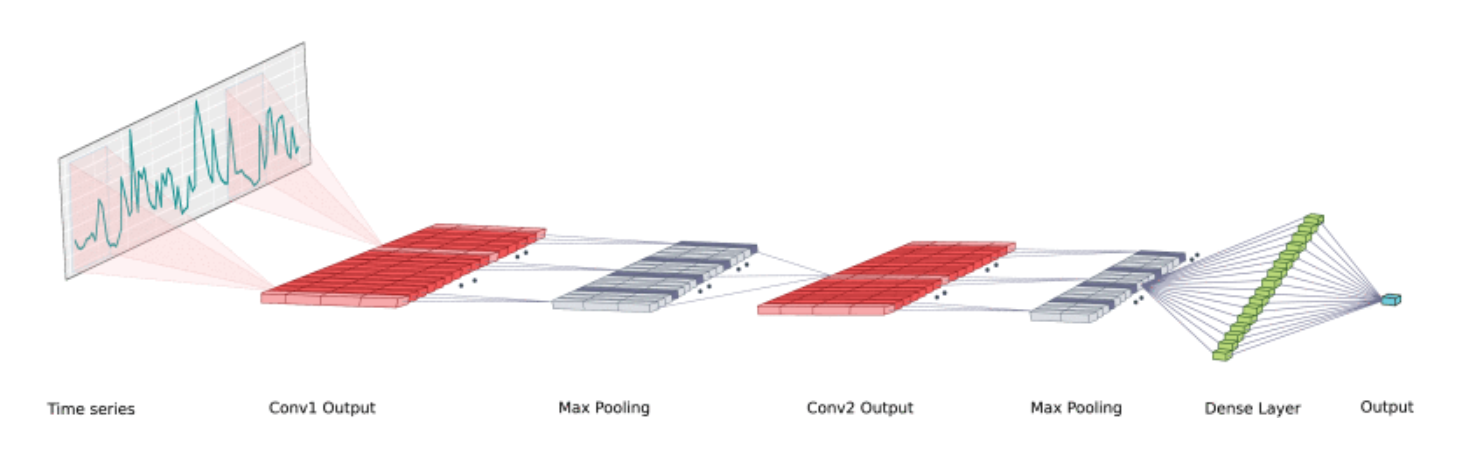
\includegraphics[scale=0.4]{Figures/CNN}
	\decoRule
	\caption[CNN Architecture for Time Series]{CNN Architecture for Time Series \parencite{Munir2019}}
	\label{fig:CNN}
	%https://ieeexplore.ieee.org/document/8581424?denied=
\end{figure}

Once the next time steps are predicted, the values are then passed to the "Anomaly Detector". The detector module calculates the Euclidian distance between the predicted and the actual data point. This measure of discrepancy is used as anomaly score. A high anomaly score indicates a significant anomaly at a given time step. In order to classify the time samples as anomalous and non-anomalous, an anomaly threshold must be specified. The anomaly threshold classifies all data points that lie under the threshold, where the Euclidean distance of predicted and actual value is small, as normal. In contrast all points that exceed the threshold are classified as anomalous. Depending on how low the threshold is set, the sensitivity can be increased \parencite{Munir2019}. In fact, such a threshold is required by all unsupervised anomaly detection algorithms. 

\clearpage
\subsection{Comparison} \label{comparison}
In an extensive study Braei and Wagner \parencite*{Braei2020} compared 20 different anomaly detection methods. The anomaly detection methods were divided into the three following  categories. 

\begin{itemize}
	\item Statistical Methods
	\item Classical Machine Learning Methods
	\item Deep Learning Based Methods (Neural Networks)
\end{itemize}


\subsubsection{Comparison of AUC}
The above stated methods were applied by Braei and Wagner \parencite*{Braei2020} on data containing point, collective and contextual anomalies. In order to compare the different approaches, AUC-Values \footnote{An ROC curve (receiver operating characteristic curve) is a graph showing the performance of a classification model at all classification thresholds. The AUC measures the entire two-dimensional area underneath the entire ROC curve. See section \ref{AUROC}} were used. The results showed that the statistical methods generally performed best on point and collective anomalies while deep learning approaches performed rather poorly. On a dataset that contained contextual anomalies, the situation reflected the exact opposite. Deep learning approaches clearly outperformed statistical methods. It was observed that deep learning approaches kept their ability to generalize while statistical methods overfitted on the data \parencite{Braei2020}.

\subsubsection{Computation Time}
The second parameter that was used to compare the different categories was training and inference time. Inference refers to the time used to classify the test data. Compared to statistical methods and classical machine learning, deep learning approaches once again performed rather poorly regarding training time. Looking at inference time deep learning approaches generally perform well, outperforming the other two categories. However, there are huge difference within the deep learning approaches. While CNNs have a very low inference time, and outperform most other algorithms, LSTMs have the highest inference time of all tested algorithms \parencite{Braei2020}.  


%https://arxiv.org/pdf/2004.00433v1.pdf
\section{Anomaly Detection on Multivariate Time Series}
In this section, anomaly detection on multivariate time series is investigated. Once again, CNNs and LSTMs are examined on the state of the art application possibilities for anomaly detection or time series classification.

\subsection{Multivariate Anomaly Detection with LSTM}
First, relevant works that use LSTMs are investigated. LSTMs will be used to establish a benchmark.

\subsubsection{Supervised Anomaly Detection using LSTM} \label{Anomaly Detection using LSTM}
In his dissertation, Alexander Verner \parencite*{Verner2019}, compared different versions of LSTM Neural Networks against traditional machine learning algorithms such as Support Vector Machines (SVM) and Random Forests. The various algorithms were applied to data of sensors that measure blood glucose levels. To measure the blood glucose levels multiple sensors are used for an accurate result, thus a multivariate time series is the outcome. The data set used in Verner's work did not contain anomalies by default, but the anomalies were embedded into the data set artificially. Since the data was also labelled after the type of anomaly it contained, the learning approach can be classified as supervised. Thus, the goal of the study was to correctly classify which anomaly was present. The first approach used a deep or stacked LSTM, with 10 units in the first layer and 35 in the second. The resulting accuracy of only 0.4 was, however, rather disappointing. This poor performance was explained with an occurring information loss within the deep network. Next, a single layer architecture, with 100 units was proposed. With just a 10\% increase the resulting accuracy was still unacceptable. In a third attempt, the neural network was enriched with an embedding layer. Using this technique, the neural network was able to detect the relationship between the frequencies of measurements that were closely positioned in the time-series. It achieved an accuracy of 98\%. The final architecture proposed by Verner \parencite*{Verner2019} then used bidirectional LSTMs (BLSTMs). According to Graves \parencite*{Graves2005}, BLSTM outperform LSTM on supervised labelling tasks. A BLSTM can extract even more information from raw data by considering the relationship of each measurement to both previous (past) and subsequent (future) measurements in the input time-series. This enhancement resulted in a 99\% accuracy. This impressive accuracy, however, comes at a cost. LSTMs are very time consuming and resource intensive to train. Verner \parencite*{Verner2019} used an Amazon Web Service computing instance with 24 CPUs, 4 GPUs and 128 GB of RAM but the training of an LSTM still took about 10 hours.  
%https://nsuworks.nova.edu/cgi/viewcontent.cgi?article=2075&context=gscis_etd

%\subsubsection{Time Series Forecasting using LSTM}
%LSTMs are normally used to forecast time series such as for example stock prices or air temperature. Following the architecture of a use case applied to a weather time series is described and investigated. The data set contains 14 different variables including air temperature, atmospheric pressure, wind direction etc. The goal in this case is to predict the air temperature as dependent variable. For this puspose a stacked GRU network was used \parencite{Chollet2018}. The above described typical use case of an RNN is relevant because it can be applied in an unsupervised learning approach. Similar as in section \ref{CNN on univariate series}, with a traditional RNN, a base could be learned to predict various time steps in the future. The time Again applying the Euclidean distance, a probability for an occurring anomaly could be calculated.
%
%
%
%
%
%
%In a first approach, a neural network using Gated Recurrent Units was proposed, in order to keep the required computation effort low. The used NN had 32 GRUs and one linear neuron in the output layer. This simple architecture was already able to outperform the established baseline, which used only used todays temperature to predict the same temperature for the next day. Since the model seemed to underfit, in a second attempt another layer with GRUs was added, to increase network capacity. The second layer was able to improve the results although not significantly. Since, the network does still not overfit the complexity could be further increased at the cost of computation time. However, a different approach was chosen. Similar as in section \ref{Anomaly Detection using LSTM} a bidirectional approach was considered. The data was therefore reversed and thus processed in antichronological order using the same network architecture as in the previous attempt. The result strongly underperformed, the established baseline indicating that a bidirectional approach would not be able to improve the results achieved with a one-directional approach. For the chosen example, it is important that data is processed in chronological order
%
%
% \parencite{Chollet2018}. 
%
%The above described typical use case of an LSTM is relevant because it can be applied in an unsupervised learning approach. Similar as in section \ref{CNN on univariate series}, with a traditional LSTM a base could be learned to predict various time steps in the future. Again applying the Euclidean distance, a probability for an occurring anomaly could be calculated.

\subsection{Multivariate Anomaly Detection with CNN}
In this section CNNs for anomaly detection but also for classification of time series are investigated. 

\subsubsection{Classification of Time Series Data using CNN}
In their research project Zheng et al. \parencite*{Zheng2014} tried to beat the state-of-the-art classification algorithm for time series, which is the k-Nearest Neighbour algorithm (k-NN). k-NN has been empirically shown to be extremely difficult to beat. The typical problem of the k-NN algorithm, however, is its computation time. Zheng et al. proposed to use their own developed architecture, which is called Multi-Channel Deep CNN (MC-DCNN). Each channel  hereby represents a CNN with convolutional and pooling layers.
Typically channels in CNN are used to extract features from the different spectra of pictures. A coloured picture for example consists of three channels, red, green and blue. Each channel now works as feature extractor on just one colour.
This feature of CNN is now used in time series classification. Every channel learns features independently using a single dimension of the multivariate time series as input. Another difference to image classification is that multivariate time series classification uses multiple 1D subsequences rather than 2D image pixels as data. Because CNN only learn features, no classification can be done. In order to classify, a CNN architecture is combined with a Multilayer Perceptron (MLP) that uses fully connected layers. Figure \ref{fig:MC-DCNN} shows the just described architecture. On the left, the different channels are shown, where every channel takes on its own univariate time series. With the denoted feature maps and pooling layers, the features of the time series are learned. In the MLP on the right, finally, the classification of the time series is done. 
It is important to note that this architecture does not predict the next time steps in the series but instead a given time series is directly classified. The classification is hereby for example used to classify the physical activity depending on the heartrate and is not used for anomaly detection. In order to use the proposed architecture for anomaly detection however, only the output layer has to be changed. 

\begin{figure}[h]
	\centering
	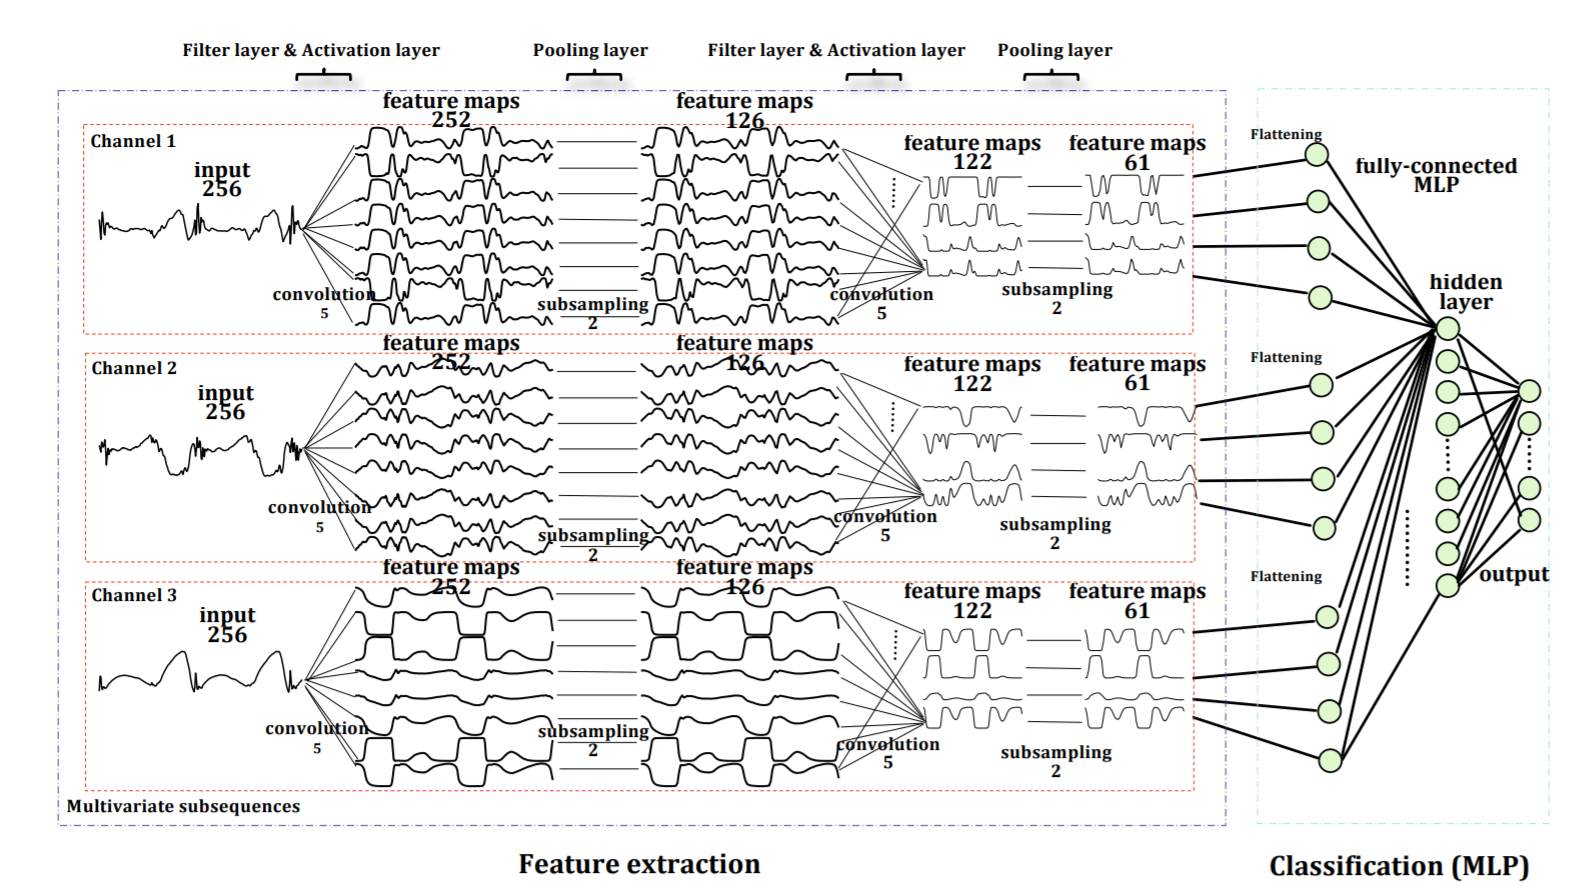
\includegraphics[scale=0.35]{Figures/MC-DCNN}
	\decoRule
	\caption[Architecture of the MC-DCNN]{Architecture of the MC-DCNN \parencite{Zheng2014}}
	\label{fig:MC-DCNN}
	%http://staff.ustc.edu.cn/~cheneh/paper_pdf/2014/Yi-Zheng-WAIM2014.pdf
\end{figure}

Zheng et al. \parencite*{Zheng2014} state that the used architecture was superior to the k-NN algorithm regarding accuracy. Further, the experiments show that deeper architecture are able to learn more robust high-level features. Further, the MC-DCNN architecture performs much faster than the k-NN algorithm, especially when a large dataset is present. The above described architecture could be adopted unchanged in order to classify anomalies.
%http://staff.ustc.edu.cn/~cheneh/paper_pdf/2014/Yi-Zheng-WAIM2014.pdf

\subsubsection{U-Nets for Anomaly Detection} \label{U-Net}
Wen and Keyes \parencite*{Wen2019} use a special type of CNN architecture to detect anomalies. The architecture used is called U-Net. A U-Net consists of so-called encoding and decoding layers. The encoding layers work like a standard CNN whereas the decoding layers are used for upsampling. Upsampling refers to restoring the previously condensed feature maps to its original size. In short, the encoding layers extract the most important features of the time series and decoding layers are using these features to assemble a new time series of the same dimensions as the original one. This encoder-decoder-architecture is often referred to as autoencoder architecture. The main weakness of autoencoders is that in the encoding part through downsampling information is permanently lost. To prevent this information loss, U-Nets introduce so called skip channels also called skip connections. A skip connection, as the name implies, is one that connects an earlier part of the network to a later part of the network and transfers data. The idea is simple: skip channels bring back missing knowledge from some earlier layers so that the network can be properly contextualized. This architecture was proven successful when applied to segmentation of neuronal structures in electron microscopic images in the original paper \parencite{Cicek2016}. In order to handle multivariate time series U-Nets also make use of multiple channels. Figure \ref{fig:U-Net} shows the architecture of the above described U-Net. The left part of the picture shows the encoding layer with five convolutional layers. The encoding layer is followed by the decoding layer, in the right part of the picture. The decoding layer consists of 4 upsampling layers. This symmetric architecture is completed by the yellow lines, that represent the skip channels.

\begin{figure}[h]
	\centering
	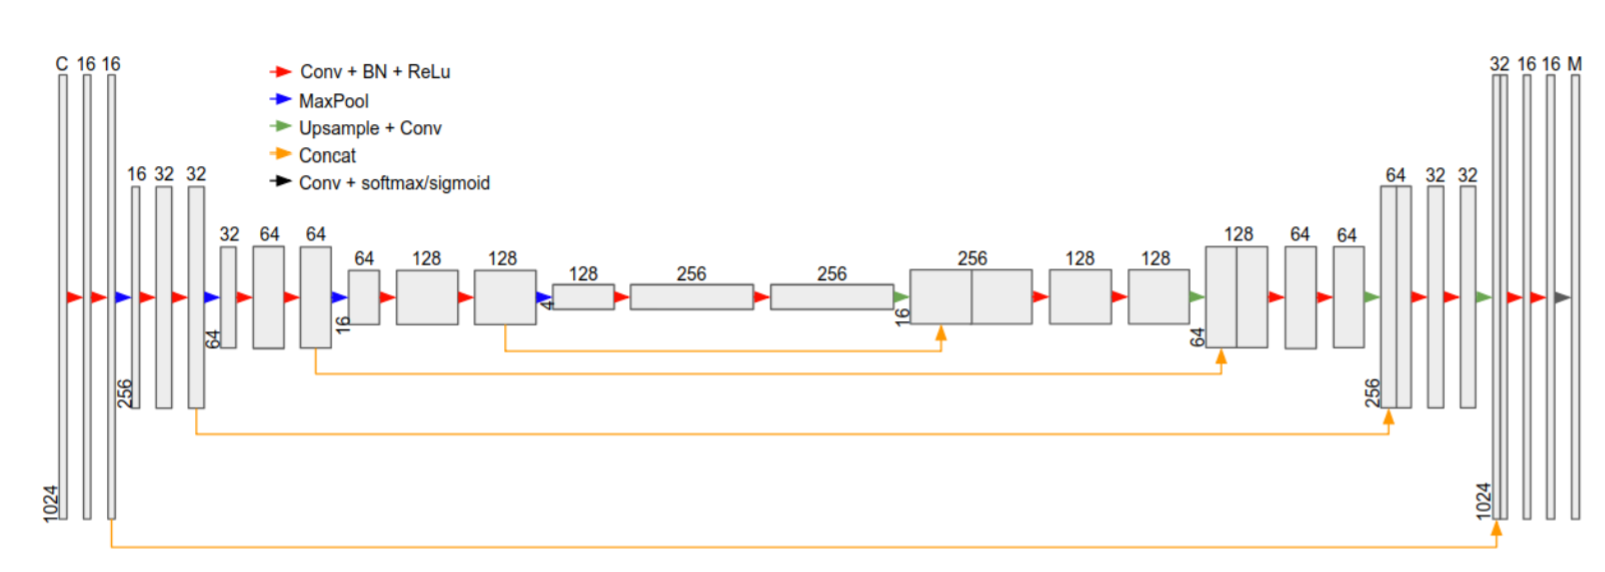
\includegraphics[scale=0.32]{Figures/U-Net}
	\decoRule
	\caption[U-Net Architecture]{U-Net Architecture \parencite{Wen2019}}
	\label{fig:U-Net}
\end{figure}

Finally, the model tries to classify what kind of anomaly the multivariate time series contained e.g a seasonal anomaly (contextual) or a point anomaly. Depending on whether the anomaly classes are mutually exclusive or not either a Sigmoid or Softmax activation is used as last layer activation function.

The proposed U-Net was tested on four scenarios: a univariate task with sufficient data, a multivariate task with sufficient data, a univariate task with insufficient data and transfer learning, and a multivariate task with insufficient data and transfer learning \parencite{Wen2019}. 

For the univariate task the dodgers loop sensor data was used. It involves a 28-week time series of traffic on a ramp near Dodger Stadium with a 5-minute frequency. The goal is to spot unusual traffic patterns caused by sporting events. Out of 39 events, only three could not be detected. The missing detection were attributed to missing values in the data set. Missing values apparently also were the reason for some false positives.

For the multivariate task the gasoil heating loop (GHL) dataset proposed by Filonov et. al \parencite*{Filonov2016} was used. It contains 48 simulated control sequences for a gasoil plant heating loop that was hacked at one stage. There are 19 variables in all time series. A multivariate U-Net with 19 channels was trained by Wen and Keyes \parencite*{Wen2019}. Out the 18, in the test present attacks, only one was missed. However, also 3 false alarms (false positives) were reported. 

%The tasks that included transfer learning are investigated further in Section \ref{TransferLearning}.

%\section{Transfer Learning} \label{Transferlearning}
%The idea behind transfer learning is to transfer knowledge from one domain to another. For example, the knowledge of a Neural Network that classifies pictures of dogs and cats can be used to classify pictures of rabbits. This is possible because all these animals share some features such as eyes or ears. Transfer learning typically uses a neural network that was pretrained on a large dataset. Some layers are then retrained on the target data set, that typically is much smaller and might not consist of enough data to train a powerful Neural Network.
%
%\subsection{Transfer Learning with CNN}
%Since CNN work as feature extractors, the idea when applying transfer learning is to transfer these features to different domains. In the first few layers a CNN typically learns low level features like corners or edges. The features are typically adopted unchanged, meaning the learned weights of the neurons are frozen. The deeper layers of CNN assemble the low level features to high level features such as an ear. Depending on how related the domain of the pretrained and the new network are, deep layers should be retrained to form other features. If a CNN that is trained to recognize animals should be used to classify furniture, the features possibly can not be adopted one-to-one. Instead, the pretrained weights of the neurons are used as initial weights compared to randomly initialised weights when training a CNN from scratch. Using this approach the CNN is fine tuned to new domain using its previous knowledge. The only part of the neural network that is trained from scratch is the classification layer at the end. This part typically consists of the fully connected layers and the output layer. These parts need to adopt to the new classes \parencite{Chollet2018}. 
%
%\subsubsection{Transfer Learning in Anomaly Detection} \label{TransferLearning}
%Wen and Keyes \parencite*{Wen2019} differentiated between transfer learning on univariate and multivariate tasks. For univariate tasks, the architecture, a U-Net, shown in Figure \ref{fig:U-Net} was used. Only the output layer was changed to match the number of classes in the target task. The pretraining was carried out with various data sets containing different kinds of anomalies such as additive outliers, anomalous temporary changes of volatility,
%and violations of cyclic patterns as these are the most common anomalies found in univariate time series. In theory, the features learned on these anomalies should be relevant for general anomaly detection. To pretrain the U-Net, synthetic time series were generated. These time series were enriched with the previously mentioned anomalies to create labelled data set for pretraining. Figure \ref{fig:Pretraing data} shows samples from the pretraining data set. In purple, additive outliers, in green changes of volatility and in red violations of cyclic patterns can be observed.
%
%\begin{figure}[h]
%	\centering
%	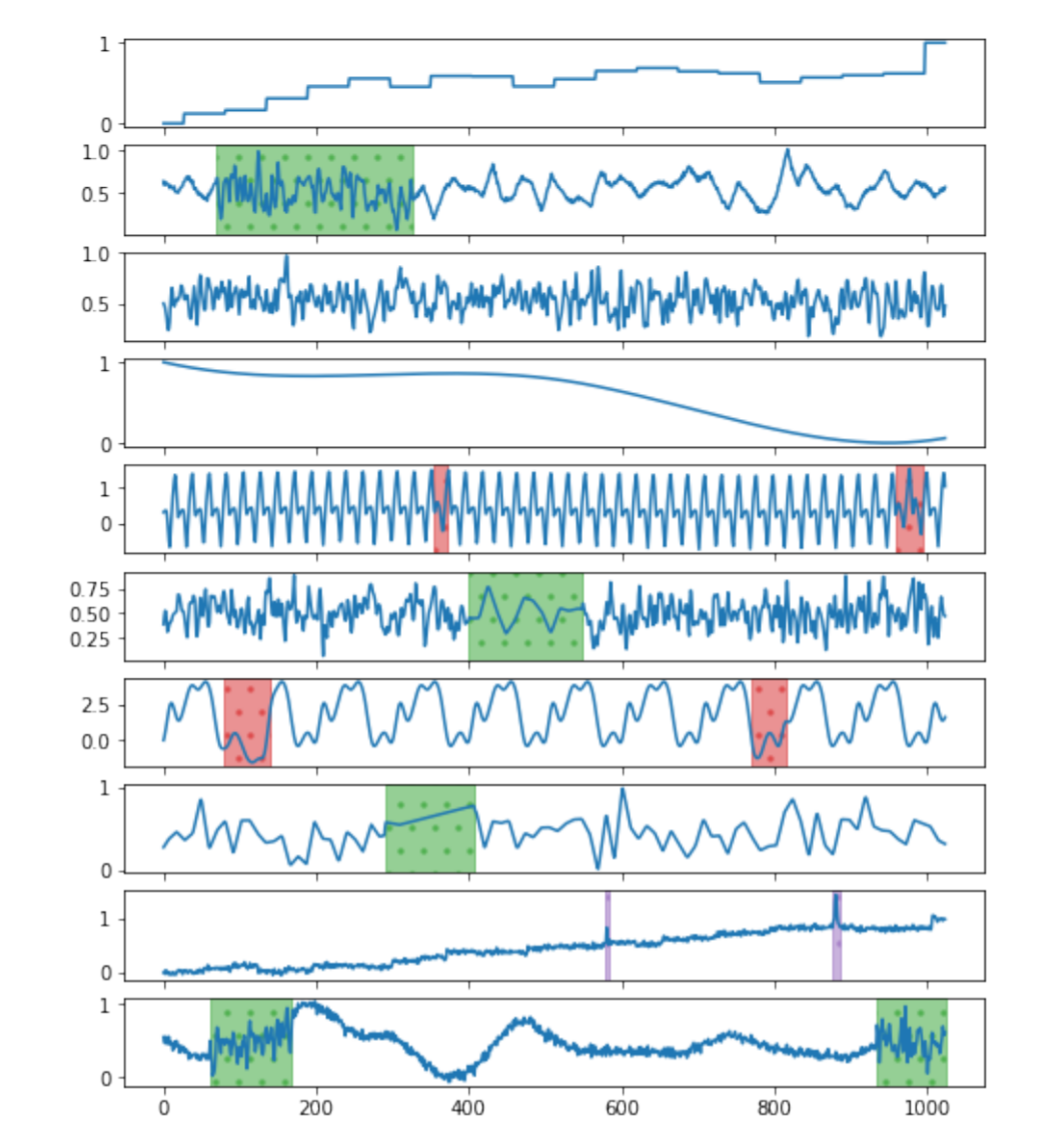
\includegraphics[scale=0.32]{Figures/Synthetic Time Series}
%	\decoRule
%	\caption[Synthetic Time Series]{Synthetic Time Series \parencite{Wen2019}}
%	\label{fig:Pretraing data}
%\end{figure}
%
%\subsection{Transfer Learning with RNN}
%Although not used as often, transfer learning can also be applied when training RNN. Similar to CNN, RNNs require large labelled data sets for training. Therefore transfer learning is valuable approach when a data set is not large enough to train a powerful RNN. When applying transfer learning, RNNs are typically trained on a related source domain, meaning the resulting weights of the neurons figure as a base. The resulting model is then fine tuned on the target domain. When applying transfer learning using RNN, better accuracy and reduced training efforts on the target domain are the main goals \parencite{Gupta2018}.
%
%%https://arxiv.org/pdf/1807.01705.pdf
%
%
%\subsubsection{Transfer Learning for Time Series Analysis}
%Gupta et al. \parencite*{Gupta2018} used a RNN trained on patient phenotypes \footnote{A clinical phenotype is the presentation of a disease in a given individual} to identify previously unseen phenotypes, but also for an unrelated task of in-hospital mortality. The idea was to train a RNN on physiological parameters to classify phenotypes. A phenotype could be the decrease in blood glucose levels. Detecting and classifying a phenotype closely resembles the task of anomaly detection.
%
%To pretrain, Gupta et al. used time series data such as glucose level or heart rate. The goal was to determine, whether a phenotype was present. Since more than one phenotype can be present, the task can be considered as multi-label classification problem. The neural network used consisted of two layers of GRUs. The output layer was designed to represent all possible phenotypes, as activation function the sigmoid function was used. This network was trained on a labelled data set.
%
%The pretrained neural network was then applied to two different target tasks. The target task was slightly reduced in complexity. Instead of a multi-label classification, the problem was formulated as a binary classification problem, determining in case a), whether or not a phenotype was present and in case b) whether a patient would survive, based on the time series observations after Intensive Care Unit (ICU) admission.
%
%
%On the target domain, training with different size data sets was done. The pretrained network was tuned on the target task with at lowest just five percent of data. As a benchmark, to compare the obtained results a logistic regression (LR) and a RNN classifier (RNN-C) were used. The two benchmarks, hereby, only operate on the target domain data set. The performances were compared using AUC (see section \ref{AUROC}) for all used algorithms per data set (Case a \& Case b).   
%
%As expected, the ROC curves of case a) showed that when the training set for the target task is small, the performance gains from transfer learning are greater. Interestingly, in case b) the benchmark RNN is able perform similarly as the two pretrained networks, indicating that better results are obtained the closer related source and target domain are.


\section{Hyperparameter Settings for fair comparison}
In this section it is investigated how CNNs and RNNs can be compared fairly. Since the two's architectures fundamentally differ it is difficult to establish a baseline, where both networks are of similar complexity. In their work Braei and Wagner \parencite*{Braei2020} chose another approach. Instead of trying to build networks with similar complexity, they fine-tuned each evaluated neural network to its full potential and compared their scores as well as their training and inference time. To compare the scores, Braei and Wagner introduced an anomaly threshold (similar as in section \ref{CNN on univariate series}). To find out the optimal threshold, it is varied to optimize sensitivity (true positive rate) and specificity (true negative rate). Varying the threshold and drawing the false positives against the true positives results in the so-called Receiver Operating Characteristics Curve (ROC-Curve), which is used to find the optimal threshold for a certain model. How the ROC-Curve is used to compare different models is explained in the next section.

\subsection{ROC and AUC} \label{AUROC}

The receiver operating characteristic curve, ROC-Curve, and the associated metric area under the curve (AUC), together also called AUROC, which is the area under the ROC-Curve, are two metrics that are frequently used to compare models. This metric is highly useful, especially for detecting anomalies. The ROC-Curve depicts the relationship between the true positive rate and the false positive rate at various threshold values \parencite{Google2021}. The variables needed for the calculations are:

\begin{itemize}
	\item TP: True Positives
	\item FN: False Negatives
	\item FP: False Positives
	\item TN: True Negatives	 
\end{itemize}

	
	The true positive rate is defined as follows: \[TPR = TP/(TP+FN)\]
	
	The false positive rate is defined as: \[FPR = FP/(FP+TN)\]

Typically, lowering the classification threshold, described in section \ref{CNN on univariate series}, causes more items to be classified as positive, which increases both False Positives and True Positives. A typical ROC curve is depicted in Figure \ref{fig:ROC}.

\begin{figure}[h]
	\centering
	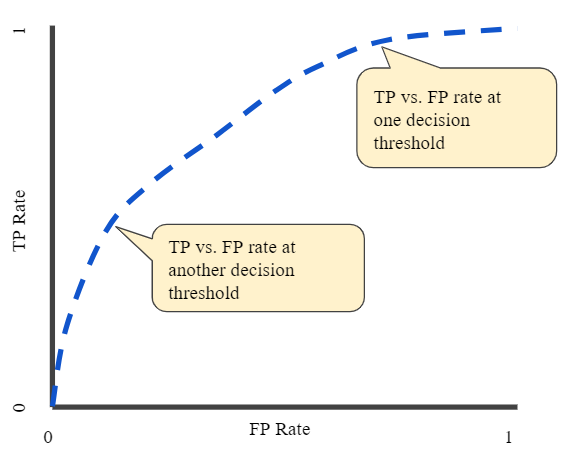
\includegraphics[scale=00.4]{Figures/ROC}
	\decoRule
	\caption[Example ROC-Curve]{Example ROC-Curve \parencite{Google2021}}
	\label{fig:ROC}
	%https://developers.google.com/machine-learning/crash-course/classification/roc-and-auc
\end{figure}

The area under the above shown curve, however, is classification-threshold-invariant. It measures the quality of the model's predictions irrespective of what classification threshold is chosen. The AUC in anomaly detection expresses the likelihood that the measured algorithm assigns a random anomalous point in the time-series a higher anomaly score than a random normal point \parencite{Google2021}. As a result, AUC is considered useful to compare different anomaly detection methods \parencite{Braei2020} .

\subsection{F-Score} 
Another approach to compare models is to use the F-Score. The F-Score describes a model's accuracy on a dataset. It is commonly used to assess binary classification systems, which categorize examples as "positive" or "negative" or in the case of anomaly detection into "anomalous" and "non-anomalous". The F-score is a method of combining the model's precision and recall, per definition it is the harmonic mean of the precision and recall of the model \parencite{Shung2018}. Precision and recall are calculated as follows from the true and false positive respectively negatives.

\[Precision = TP/(FP+TP)\]
\[Recall = TP/(TP+FN)\]

From precision and recall the F-Score, and in this specific case the F1-Score can be calculated as follows.

\[F1 = 2*(Precision*Recall)/(Precision+Recall)\]

When applying the F-Score, a perfect model has a score of 1. Therefore, different models can also easily be compared. In his dissertation, Verner \parencite*{Verner2019}, used the F1-Score to asses different anomaly detection methods.


\subsection{Computation Time}
Another approach to compare the performances is to compare the computation times. To compare the computation times Braei and Wagner \parencite*{Braei2020} looked at the average training and inference time of traditional machine learning models as well as  statistical models and neural networks on univariate time series. Generally, neural networks are expected to invest most of their computation time in training and are able to outperform the traditional machine learning on inference time. However, the practical results showed that Recurrent Neural Networks (LSTM \& GRU) not only needed a long time to train but also had a large inference time on certain data sets. With LSTM performing second best on the given data set, behind k-means clustering, it can be concluded that this comes with a trade-off. On the same data set a CNN was trained. The CNN achieved an AUC-Value of 0.818, compared to 0,84 of the LSTM, which is not much worse than LSTM. Looking at the training and inference time, the CNN is superior. The LSTM takes about 1000 seconds for training and also inference. The CNN, however, trains for 50 seconds, with an inference time of under one second, making the CNN the better choice, when relying on small inference times \parencite{Braei2020}.

\section{Research Gap}
Anomaly detection on time series data has been widely researched. There are comprehensive comparisons of statistical methods, traditional machine learning approaches and neural networks such as the works of Braei and Wagner \parencite*{Braei2020} or Verner \parencite*{Verner2019}. Braei and Wager \parencite*{Braei2020}, focus thereby only on univariate time series. Complementary, Verner \parencite*{Verner2019} only investigated multivariate time series. In their work, Braei and Wagner \parencite*{Braei2020} could show that CNN and RNN are able to achieve similar performances, while CNNs are superior in computation time. Verner \parencite*{Verner2019} faced a similar drawback in his research, where the training of the RNN took approximately 10 hours. 

Since CNNs are only very recently investigated for anomaly detection in time series, Verner \parencite*{Verner2019} did not include them in his research. The approaches presented by Zheng et al. \parencite*{Zheng2014} and Wen and Keyes \parencite*{Wen2019}, however, show promising results, when using CNNs for time series classification respectively anomaly detection. 

As research gap it has been identified that is currently unknown if CNNs are able to outperform RNNs when used in the field of anomaly detection. Braei and Wagner \parencite*{Braei2020} were already able to achieve good results when testing the approach on univariate time series. This work attempts to extend this knowledge to multivariate time series.
%As research gap it has been identified that there is currently no research on how well CNNs perform when used in the field of anomaly detection. The works mentioned above do not establish a state of the art baseline, to compare the achieved results. It is therefore currently not assessable, how useful CNNs are for anomaly detection.

%Further, since the use of neural networks steadily increases, it can be anticipated that transfer learning approaches that save training time, improve accuracy and are able to deal with small data sets will become more popular. Both papers, that compare the different methods for anomaly detection do not take advantage of this approach.

